\documentclass{beamer}

\mode<presentation> {
	\usetheme{Berlin}
}

\title[12th International Conference on Large-Scale Scientific Computations, June 10 - 14, 2019, Sozopol, Bulgaria]{
	Solving Combinatorial Puzzles with Parallel Evolutionary Algorithms
}

\author{Todor Balabanov, Stoyan Ivanov, Rumen Ketipov}

\date{10-14.VI.2019}

\institute[IICT-BAS, LSSC'19] {
	Institute of Information and Communication Technologies \\ 
	Bulgarian Academy of Sciences \\
	\medskip
	\textit{todorb@iinf.bas.bg}
}

\begin{document}

\begin{frame}
\titlepage
\end{frame}

\begin{frame}
\frametitle{Overview}
\tableofcontents
\end{frame}

\section{Introduction}

\begin{frame}
\center \huge{Introduction}
\end{frame}

\begin{frame}
\frametitle{Rubik's Cube}
\begin{itemize}
  \item Invented and introduced by Erno Rubik in the 70s
  \item The most popular combinatorial puzzle all over the world
  \item It has 3x3x3 cubical segments
  \item Six different colors on each subcube square of the exposed sides
  \item Each of the six planes (3x3x1) can be rotated in 90, 180, 270 or 360 degrees
  \item As initial state all sides of the cube are in single color
  \item Scumbling of the puzzle is done by many random rotations
  \item The goal is to restore the cube in its original state
\end{itemize}
\end{frame}

\begin{frame}
\frametitle{Genetic Algorithms}
\begin{itemize}
  \item Global optimization strategy
  \item Inspired by the natural evolution
  \item Solutions are represented as vectors (individual) of values into the solution space
  \item Initial population is initialized randomly
  \item Each new generation is created by selection and recombination
  \item Suitable for parallel implementation
\end{itemize}
\end{frame}

\section{Proposed Rubik's Cube Solver}

\begin{frame}
\center \huge{Proposed Rubik's Cube Solver}
\end{frame}

\begin{frame}
\frametitle{Data Structures}
\begin{itemize}
  \item The cube is presented as six (one for each side) two-dimensional (3x3) arrays
  \item Values in the arrays are integer numbers corresponding to cube's colors
  \item Six common operations over the cube sides are defined
\end{itemize}
\end{frame}

\begin{frame}
\frametitle{Minimal Fully Functional Grammar}
\begin{itemize}
  \item T (Top) –90 degrees clockwise rotation of the top side
  \item L (Left) –90 degrees clockwise rotation of the left side
  \item B (Back) –90 degrees clockwise rotation of the back side
  \item R (Right) –90 degrees clockwise rotation of the right side
  \item F (Front) –90 degrees clockwise rotation of the front side
  \item D (Down) –90 degrees clockwise rotation of the down side
\end{itemize}
\end{frame}

\begin{frame}
\frametitle{Extended Grammars}
\begin{itemize}
  \item Counter-clockwise operators included: \\
  +T, +L, +B, +R, +F, +D, -T, -L, -B, -R, -F, -D
  \item Number of turns included: \\
  +1T, +2T, +3T, +1L, +2L, +3L, +1B, +2B, +3B, +1R, +2R, +3R, +1F, +2F, +3F, +1D,+2D, +3D, -1T, -2T, -3T, -1L, -2L, -3L, -1B, -2B, -3B, -1R, -2R, -3R, -1F, -2F, -3F, -1D, -2D, -3D
\end{itemize}
\end{frame}

\begin{frame}
\frametitle{Individuals Representation}
\begin{itemize}
  \item Formal grammar sentences with variable length
  \item Each of the operations can appear at any position many times
  \item The average expected length of the chromosomes is between 50 and 100
\end{itemize}
\end{frame}

\begin{frame}
\frametitle{Recombination Parameters}
\begin{itemize}
  \item Single cut point crossover
  \item Random change of a single instruction mutation
  \item Random selection of parents
  \item Elitism rule
\end{itemize}
\end{frame}

\begin{frame}
\frametitle{Fitness Value}
\begin{itemize}
  \item Instructions from GA individual are applied over the scrambled cube
  \item Hausdorff distance between manipulated cube and solved cube is calculated
  \item Lower fitness values are for better individuals
\end{itemize}
\end{frame}

\begin{frame}
\frametitle{Proposed Fitness Evaluation}
\begin{figure}[h]
  \centering
  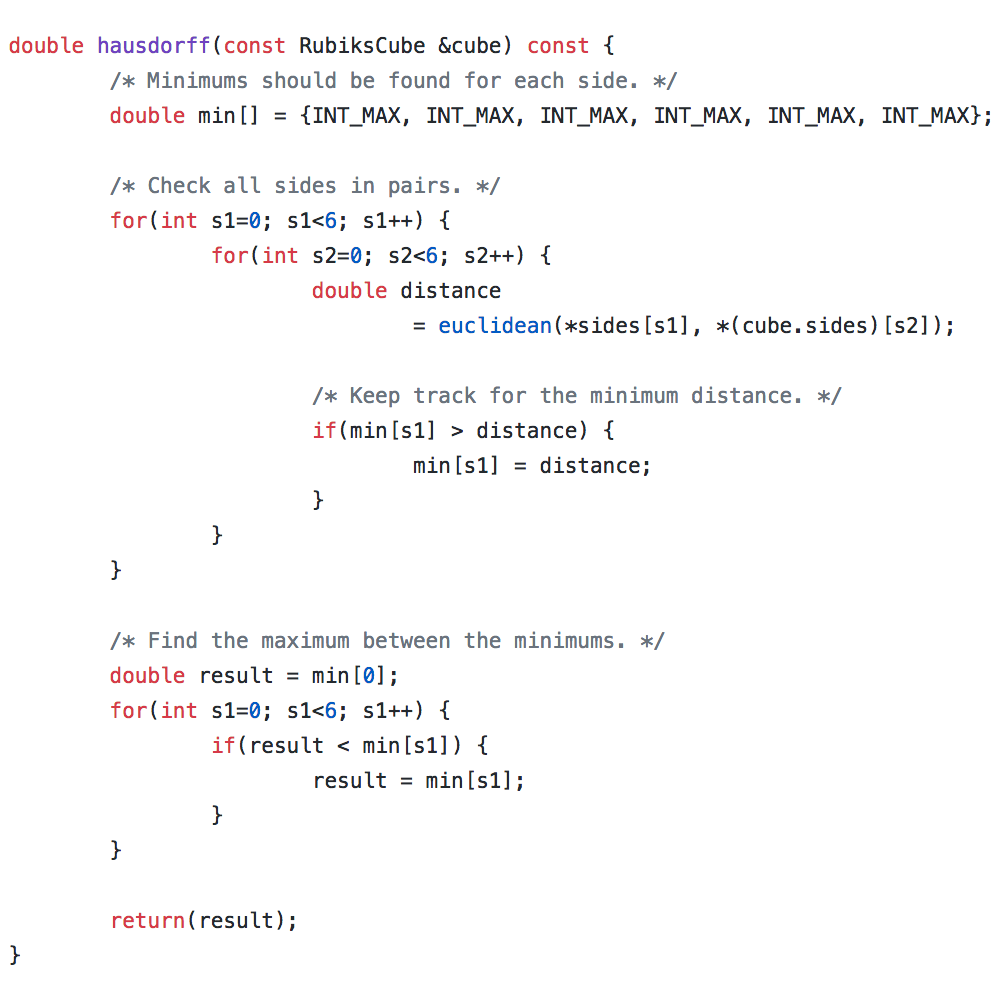
\includegraphics[width=1.0\textwidth,height=0.65\textwidth]{fig01}
  \label{fig01}
\end{figure}
\end{frame}

\section{Experiments and Results}

\begin{frame}
\center \huge{Experiments and Results}
\end{frame}

\begin{frame}
\frametitle{Platform Setup}
\begin{itemize}
  \item Intel Core i5, 2.3 GHz, 2 Cores, 8GB RAM
  \item Mac OS X 10.13.6
  \item Apple LLVM version 9.1.0 / Open MPI
\end{itemize}
\end{frame}

\begin{frame}
\frametitle{Genetic Algorithm Parameters}
\begin{itemize}
  \item Generation gap: 0.93
  \item Crossover rate: 0.98
  \item Mutation rate: 0.01
  \item Maximum generations: 10000
  \item Number of individuals: 37
  \item Number of variables: floating
  \item Inserted rate: 100
\end{itemize}
\end{frame}

\begin{frame}
\frametitle{Star Topology Results}
\begin{figure}[h]
  \centering
  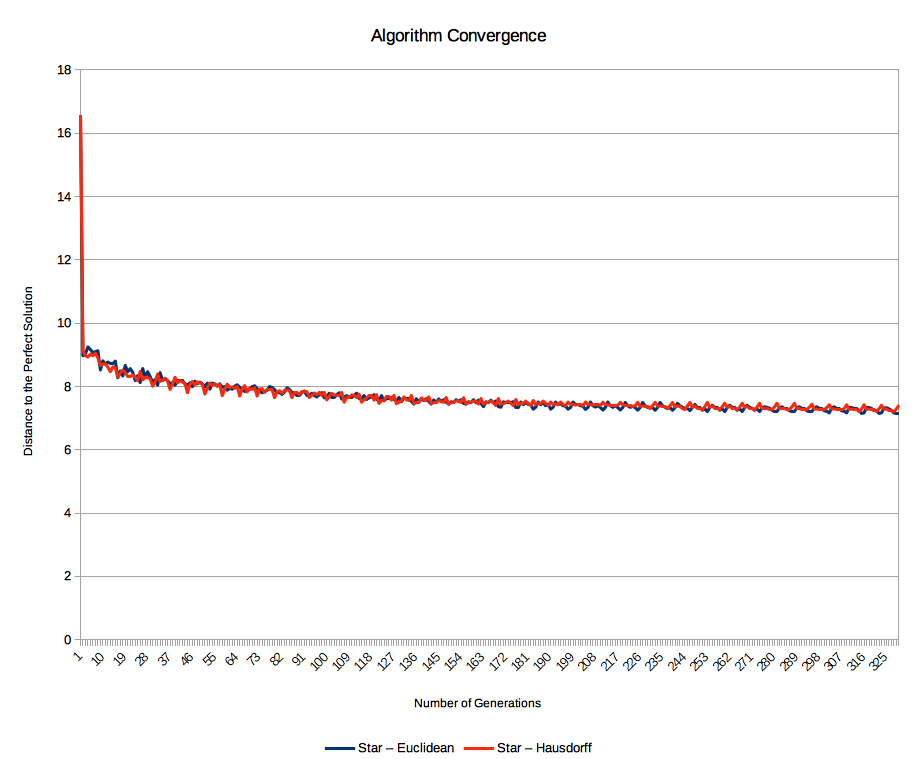
\includegraphics[width=1.0\textwidth,height=0.5\textwidth]{fig03}
  \label{fig03}
\end{figure}
\end{frame}

\begin{frame}
\frametitle{Incident Nodes Participation}
\begin{figure}[h]
  \centering
  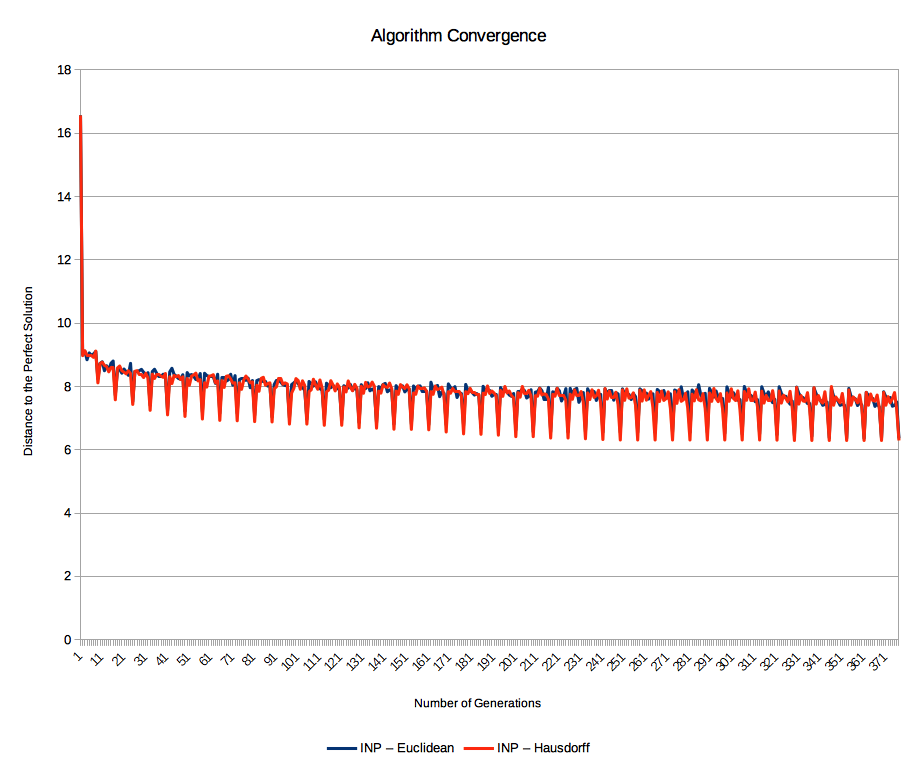
\includegraphics[width=1.0\textwidth,height=0.5\textwidth]{fig04}
  \label{fig04}
\end{figure}
\end{frame}

\section{Conclusions}

\begin{frame}
\center \huge{Conclusions}
\end{frame}

\begin{frame}
\frametitle{Concluding Remarks}
\begin{itemize}
  \item Addition of Hausdorff distance component improves the performance of the genetic algorithm
  \item Calculation of the Hausdorff distance is a little bit slower than the calculation of the Euclidean distance
  \item Better solution fitness estimation generally leads to genetic algorithm convergence improvement
\end{itemize}
\end{frame}

\begin{frame}
\frametitle{Questions and Answers}
\center \huge{Thank you for the attention!}
\end{frame}

\end{document}
